% Choose one to switch betweeen slides and handout
%\documentclass[]{beamer}
\documentclass[handout]{beamer}

% Video Meta Data
\title{Bitcoin, Blockchain and Cryptoassets}
\subtitle{Economic Scripting}
\author{Prof. Dr. Fabian Schär}
\institute{University of Basel}

% Config File
% Packages
\usepackage[utf8]{inputenc}
\usepackage{hyperref}
\usepackage{gitinfo2}
\usepackage{tikz}
\usepackage{amsmath}
\usepackage{bibentry}
\usepackage{xcolor}
\usepackage{colortbl} % Add colour to LaTeX tables
\usepackage{caption}
\usepackage[export]{adjustbox}
\usepackage{pgfplots} \pgfplotsset{compat = 1.17}

% Color Options
\definecolor{highlight}{rgb}{0.65,0.84,0.82}
\definecolor{focus}{rgb}{0.72, 0, 0}

% Beamer Template Options
\beamertemplatenavigationsymbolsempty
\setbeamertemplate{footline}[frame number]
\setbeamercolor{structure}{fg=black}
\setbeamercolor{footline}{fg=black}
\setbeamercolor{title}{fg=black}
\setbeamercolor{frametitle}{fg=black}
\setbeamercolor{item}{fg=black}
\setbeamercolor{}{fg=black}
\setbeamercolor{bibliography item}{fg=black}
\setbeamercolor*{bibliography entry title}{fg=black}
\setbeamertemplate{items}[square]
\setbeamertemplate{enumerate items}[default]
\captionsetup[figure]{labelfont={color=black},font={color=black}}
\captionsetup[table]{labelfont={color=black},font={color=black}}

\setbeamertemplate{bibliography item}{\insertbiblabel}

% Link Icon Command
\newcommand{\link}{%
    \tikz[x=1.2ex, y=1.2ex, baseline=-0.05ex]{%
        \begin{scope}[x=1ex, y=1ex]
            \clip (-0.1,-0.1)
                --++ (-0, 1.2)
                --++ (0.6, 0)
                --++ (0, -0.6)
                --++ (0.6, 0)
                --++ (0, -1);
            \path[draw,
                line width = 0.5,
                rounded corners=0.5]
                (0,0) rectangle (1,1);
        \end{scope}
        \path[draw, line width = 0.5] (0.5, 0.5)
            -- (1, 1);
        \path[draw, line width = 0.5] (0.6, 1)
            -- (1, 1) -- (1, 0.6);
        }
    }

% Read Git Data from Github Actions Workflow
% Defaults to gitinfo2 for local builds
\IfFileExists{gitInfo.txt}
	{\input{gitInfo.txt}}
	{
		\newcommand{\gitRelease}{(Local Release)}
		\newcommand{\gitSHA}{\gitHash}
		\newcommand{\gitDate}{\gitAuthorIsoDate}
	}

% Custom Titlepage
\defbeamertemplate*{title page}{customized}[1][]
{
  \vspace{-0cm}\hfill
\includegraphics[width=2.5cm]{../config/logo_cif}
  
\includegraphics[width=1.9cm]{../config/seal_wwz}
  \\ \vspace{2em}
  \usebeamerfont{title}\textbf{\inserttitle}\par
  \usebeamerfont{title}\usebeamercolor[fg]{title}\insertsubtitle\par  \vspace{1.5em}
  \small\usebeamerfont{author}\insertauthor\par
  \usebeamerfont{author}\insertinstitute\par \vspace{2em}
  \usebeamercolor[fg]{titlegraphic}\inserttitlegraphic
    \tiny \noindent \texttt{Release Ver.: \gitRelease}\\ 
    \texttt{Version Hash: \gitSHA}\\
    \texttt{Version Date: \gitDate}\\ \vspace{1em}
  \link \href{https://github.com/cifunibas/Bitcoin-Blockchain-Cryptoassets/blob/main/slides/intro.pdf}
  {Get most recent version}\\
  \link \href{https://github.com/cifunibas/Bitcoin-Blockchain-Cryptoassets/blob/main/slides/intro.pdf}
  {Watch video lecture}\\ \vspace{1em}
  License: \texttt{Creative Commons Attribution-NonCommercial-ShareAlike 4.0 International}\\\vspace{2em}
  
\includegraphics[width = 1.2cm]{../config/license}
}

% tikzlibraries
\usetikzlibrary{decorations.pathreplacing}
\usetikzlibrary{decorations.markings}
\usetikzlibrary{positioning}

%caption font
\captionsetup{font=footnotesize}


% Other Inputs
% Defining Bitcoin Symbol
\def\btc{%
	\leavevmode
	\vtop{\offinterlineskip %\bfseries
		\setbox0=\hbox{B}%
		\setbox2=\hbox to\wd0{\hfil\hskip-.03em
			\vrule height .3ex width .15ex\hskip .08em
			\vrule height .3ex width .15ex\hfil}
		\vbox{\copy2\box0}\box2}}
% Definition of a green checkmark symbol
% Code based on: https://tex.stackexchange.com/questions/532033/make-a-double-blue-checkmark-symbol-with-square-contours-using-tikz

% Create shape of a green checkmark
\tikzset{pics/.cd, checkmark/.style={code={% 
			\pgfgettransformentries{\tmpxx}{\tmp}{\tmp}{\tmp}{\tmp}{\tmp}
			\draw[line width=\tmpxx*1pt,draw=none,fill=green!60] (0,.33) -- (.25,0) to 
			(0.8,.6) to (.72,.68) to (.25,.18) to (0.08,.40)-- cycle;}}}

\newcommand{\checkmarkgreen}{
\begin{tikzpicture}[baseline={(0,0)}]
		\path (0,0) pic[scale=1]{checkmark};
\end{tikzpicture}}



%%%%%%%%%%%%%%%%%%%%%%%%%%%%%%%%%%%%%%%%%%%%%%
%%%%%%%%%%%%%%%%%%%%%%%%%%%%%%%%%%%%%%%%%%%%%%
\begin{document}

\thispagestyle{empty}
\begin{frame}[noframenumbering]
	\titlepage
\end{frame}

%%%

\begin{frame}{Transactions Review}
	What has been covered so far:
	\begin{itemize}
		\item<1 -> Transaction types
		\begin{itemize}
			\item<1 -> Pay-to-Address, Pay-to-Multisig, Pay-to-Script-Hash, etc.
		\end{itemize}
		\item<2 -> Signature hash types
		\begin{itemize}
			\item<2 -> \texttt{SIGHASH\_ALL}, \texttt{SIGHASH\_NONE|SIGHASH\_ANYONECANPAY}, etc.
		\end{itemize}
		\item<3 -> Using these components and clever transaction design, smart contracts can be implemented on the Bitcoin Blockchain.
	\end{itemize}
\end{frame}

%%%

\begin{frame}{Further Scripting Components}
	\begin{itemize}
		\item<1-> \textbf{Timelocks}
		\begin{itemize}
			\item<1-> Lock a transaction or output for a relative or absolute point in time.
		\end{itemize}
		\vspace{0.25cm}
		\item<2-> \textbf{Competitive Outputs}
		\begin{itemize}
			\item<2-> Two competing options to use one single output.
		\end{itemize}
		\vspace{0.25cm}
		\item<3-> \textbf{Hashlocks}
		\begin{itemize}
			\item<3-> Require the knowledge of some secret input in order to spend an output.
		\end{itemize}
	\end{itemize}
\end{frame}

%%%

\begin{frame}{Timelocks}
	\begin{itemize}
		\item<1-> UTXOs can be locked for a specified time
		\begin{itemize}
			\item<1-> Absolute timelocks use a specific point in time or block height (analogy: "at 12 o'clock").
			\item<1-> Relative timelocks specify a number of blocks after confirmation (analogy: "in five hours").
		\end{itemize}
		\item<2 -> Four alternatives for implementation
	\end{itemize}
	\vspace{0.25cm}
	\uncover<2->{\begin{table}
			\center
			\resizebox{\textwidth}{!}{%
				\begin{tabular}{lll} \hline \hline
					& Transaction level     & Output level\\
					\cline{2-3}
					& Consensus             & Scripting Language\\ \hline
					Absolute timelock  & \texttt{nLockTime}    & CHECKLOCKTIMEVERIFY (CLTV)\\ 
					Relative timelock  & \texttt{nSequence}    & CHECKSEQUENCEVERIFY (CSV)\\\hline \hline
			\end{tabular}}
	\end{table}}
\end{frame}

%%%

\begin{frame}{Competitive Outputs}
	\begin{minipage}{0.3\textwidth}
		\begin{figure}
			\begin{tikzpicture}
				[scale=0.9, every node/.style={scale=0.9}]
				% Structure
				\filldraw[yshift=-0.05cm, xshift=0.1cm,color = highlight!15, thick, 	draw=black, dashed] (0.95,-5.8) rectangle ++(4cm,4.9cm);
				\filldraw[yshift=-0.05cm, xshift=0.1cm,color = highlight!25, thick, draw=highlight] (1.3,-5.4) rectangle ++(3.3cm,3.8cm);
				\draw[color=black, thick, dashed] (1.6,-3.75) -- (4.4,-3.75);
				
				% Outputs
				\draw[color=black] plot (3,-1.65)   node[above] {\texttt{outputs:}};
				
				
				% top
				\filldraw[yshift=-0.05cm, xshift=0.1cm,color = highlight!25, thick, 	draw=highlight] (1.3,-3.4) rectangle ++(0.825cm,0.7cm);
				\filldraw[yshift=-0.05cm, xshift=0.1cm,color = highlight!25, thick, 	draw=highlight] (2.125,-3.4) rectangle ++(0.825cm,0.7cm);
				
				\draw[color=black] plot (1.4,-2.25)   node[right] {Multisig:};
				\draw[color=black] plot (3.3,-2.25)   node[right] {2 BTC};
				\draw[color=black] plot (1.8125,-3.1)   node {\small{$Sig_A$}};
				\draw[color=black] plot (2.6375,-3.1)   node {\small{$Sig_B$}};
				
				% bottom
				\filldraw[yshift=-0.05cm, xshift=0.1cm,color = highlight!25, thick,draw=highlight] (1.3,-5.4) rectangle ++(0.825cm,0.7cm);
				\filldraw[yshift=-0.05cm, xshift=0.1cm,color = highlight!25, thick,draw=highlight] (2.125,-5.4) rectangle ++(0.825cm,0.7cm);
				
				\draw[color=black] plot (1.4,-4.25)   node[right] {Alice:};
				\draw[color=black] plot (3.3,-4.25)   node[right] {2 BTC};
				\draw[color=black] plot (1.8125,-5.1)   node {\small{$Sig_A$}};
				\draw[color=black] plot (2.6375,-5.1)   node {
\includegraphics[width=0.5cm]{../assets/images/timelock_symbol.png}};
			\end{tikzpicture}
		\end{figure}
	\end{minipage}%
	\hfill
	\begin{minipage}{0.6\textwidth}
		\begin{itemize}
			\item<1-> Two options, only one needed to spend the output.
			\item<2-> Output can only be spent once. The two options are competitive.
			\vspace{0.25cm}
			\item<3-> \textbf{Example:}
			\begin{itemize}
				\item<3-> Output can be spend by Alice and Bob (Multisig) as soon as the transaction is confirmed.
				\item<4-> After a specific point in time (CLTV) Alice has the option to spend unilaterally.
			\end{itemize}
		\end{itemize}
	\end{minipage}
\end{frame}

%%%

\begin{frame}{Hashlocks}
	\begin{itemize}
		\item<1-> Outputs can be (additionally) tied to the disclosure of a specific piece of data ($m$).
		\item<2-> Hash value $\left(h = H(m)\right)$ of the secret input is recorded in the transaction.
	\end{itemize}
	\uncover<3->{\begin{figure}[b]
		\begin{tikzpicture}[scale=0.9, every node/.style={scale=0.9}]
			\filldraw[yshift=-0.05cm, xshift=0.1cm,color = highlight!15, thick, 	draw=black, dashed] (-3,-3.6) rectangle ++(8cm,2.6cm);
			
			\draw[color=black] plot (1,-0.4) node [below]
			{\large{{Hashlock Transaction}}};
			
			% Inputs
			\draw[color=black] plot (-1,-1.65) node[above] {\texttt{inputs:}};
			
			% top left
			\filldraw[yshift=-0.05cm, xshift=0.1cm,color = highlight!25, thick, 	draw=highlight] (-2.6,-3.4) rectangle ++(3.3cm,1.8cm);
			\filldraw[yshift=-0.05cm, xshift=0.1cm,color = highlight!25, thick, 	draw=highlight] (-2.6,-3.4) rectangle ++(0.825cm,0.7cm);
			\draw[color=black] plot (-2.5,-2.25) node[right] {Alice:};
			\draw[color=black] plot (-0.6,-2.25)   node[right] {1 BTC};
			\draw[color=black] plot (-2.0875,-3.1)   node {\small{$Sig_A$}};
			
			\draw plot (-2.1,-3.1) node {\checkmarkgreen};
			
			% Outputs
			\draw[color=black] plot (3,-1.65)   node[above] {\texttt{outputs:}};
			
			% top right
			\filldraw[yshift=-0.05cm, xshift=0.1cm,color = highlight!25, thick, draw=highlight] (1.3,-3.4) rectangle ++(3.3cm,1.8cm);
			\filldraw[yshift=-0.05cm, xshift=0.1cm,color = highlight!25, thick, 	draw=highlight] (1.3,-3.4) rectangle ++(0.825cm,0.7cm);
			\filldraw[yshift=-0.05cm, xshift=0.1cm,color = highlight!25, thick, 	draw=highlight] (2.125,-3.4) rectangle ++(0.825cm,0.7cm);
			\draw[color=black] plot (1.4,-2.25)   node[right] {Bob:};
			\draw[color=black] plot (3.3,-2.25)   node[right] {1 BTC};
			\draw[color=black] plot (1.8125,-3.1)   node {\small{$Sig_B$}};
			\draw[color=black] plot (2.6375,-3.1)   node {
\includegraphics[width=0.5cm]{../assets/images/hashlock_symbol.png}};
		\end{tikzpicture}
	\end{figure}}
	\begin{itemize}
		\item<4-> UTXO can only be spend if one can present a piece of data which results in the same hash value (i.e., if Alice tells Bob the secret ($m$)).
	\end{itemize}
\end{frame}

%%%

\begin{frame}{Hashlocks}
	\begin{minipage}{0.1\linewidth}
		\vspace{0.3cm}
		\centering
		
\includegraphics[width=1cm]{../assets/images/agents/handing_right}
		\\ \hspace{-0.3cm} \textbf{Alice}\\
		\vspace{0.3cm}
		\uncover<1->{
		\hspace{-0.2cm}	
\includegraphics[width=1cm]{../assets/images/hashlock_symbol}
		}
	\end{minipage}%
	\begin{minipage}{0.8\linewidth}
	\uncover<2->{\begin{figure}[b]
					\begin{tikzpicture}[scale=0.9, every node/.style={scale=0.9}]
						\filldraw[yshift=-0.05cm, xshift=0.1cm,color = highlight!15, thick, 	draw=black, dashed] (-3,-3.6) rectangle ++(8cm,2.6cm);
						
						\draw[color=black] plot (1,-0.4) node [below]
						{\large{{Hashlock Transaction}}};
						
						% Inputs
						\draw[color=black] plot (-1,-1.65) node[above] {\texttt{inputs:}};
						
						% top left
						\filldraw[yshift=-0.05cm, xshift=0.1cm,color = highlight!25, thick, 	draw=highlight] (-2.6,-3.4) rectangle ++(3.3cm,1.8cm);
						\filldraw[yshift=-0.05cm, xshift=0.1cm,color = highlight!25, thick, 	draw=highlight] (-2.6,-3.4) rectangle ++(0.825cm,0.7cm);
						\draw[color=black] plot (-2.5,-2.25) node[right] {Alice:};
						\draw[color=black] plot (-0.6,-2.25)   node[right] {1 BTC};
						\draw[color=black] plot (-2.0875,-3.1)   node {\small{$Sig_A$}};
						
						\draw plot (-2.1,-3.1) node {\checkmarkgreen};
						
						% Outputs
						\draw[color=black] plot (3,-1.65)   node[above] {\texttt{outputs:}};
						
						% top right
						\filldraw[yshift=-0.05cm, xshift=0.1cm,color = highlight!25, thick, draw=highlight] (1.3,-3.4) rectangle ++(3.3cm,1.8cm);
						\filldraw[yshift=-0.05cm, xshift=0.1cm,color = highlight!25, thick, 	draw=highlight] (1.3,-3.4) rectangle ++(0.825cm,0.7cm);
						\filldraw[yshift=-0.05cm, xshift=0.1cm,color = highlight!25, thick, 	draw=highlight] (2.125,-3.4) rectangle ++(0.825cm,0.7cm);
						\draw[color=black] plot (1.4,-2.25)   node[right] {Bob:};
						\draw[color=black] plot (3.3,-2.25)   node[right] {1 BTC};
						\draw[color=black] plot (1.8125,-3.1)   node {\small{$Sig_B$}};
						\draw[color=black] plot (2.6375,-3.1)   node {
\includegraphics[width=0.5cm]{../assets/images/hashlock_symbol.png}};
					\end{tikzpicture}
		\end{figure}}
	\end{minipage}%
	\begin{minipage}{0.1\linewidth}
		\vspace{0.82cm}
		\centering
		\hspace{-0.2cm}
\includegraphics[width=1cm]{../assets/images/agents/handing_left}
		\\ \textbf{Bob}\\
		\vspace{0.3cm}
		\uncover<3->{
		
\includegraphics[width=1cm]{../assets/images/hashlock_symbol}
			}
	\end{minipage}
	\begin{itemize}
		\item<4 -> Powerful in combination with other conditions or when secret unlocks outputs on more than one Blockchain.
	\end{itemize}
\end{frame}

%%%

\begin{frame}{Hash Time Locked Contracts (HTLC)}
	\textbf{Generally:}
	\begin{itemize}
		\item<1-> HTLC consist of combinations of timelocks and hashlocks. They are usually used for cross chain swaps and payment channels.
	\end{itemize}
	\vspace{0.5cm}
	\uncover<2->{\textbf{Example: Atomic Cross Chain Swaps}}
	\begin{itemize}
		\item<2-> Two Blockchains, {A-Chain} and {B-Chain}, with native assets \texttt{A-Coin} and \texttt{B-Coin}, respectively. 
		\item<3-> Alice wants to swap 2 \texttt{B-Coins} for one of Bob's \texttt{A-Coins}.
		\item<4-> Counterparty risk...
		\item<5-> Solution: Creation of one transaction on each Blockchain, both s.t. the same secret hashlock.
		\item<6-> Once secret is revealed, both transactions are spendable.
	\end{itemize}
\end{frame}

%%%

\begin{frame}{Atomic Cross Chain Swaps}
	\begin{minipage}{0.1\linewidth}
		\vspace{0.6cm}
		\centering
		
\includegraphics[width=1cm]{../assets/images/agents/handing_right}
		\\ \hspace{-0.3cm} \textbf{Alice}\\
		\vspace{0.3cm}
		\tikz{\filldraw[color = white!1] (0,0) rectangle ++(1cm,1cm);}
	\end{minipage}%
	\begin{minipage}{0.8\linewidth}
		\centering
		\begin{figure}[t]
			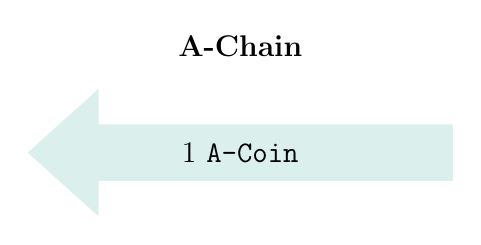
\begin{tikzpicture}[scale=0.9, every node/.style={scale=0.9}]
				\draw[color=black] plot (0,1.5) node {\large{{\textbf{A-Chain}}}};
				\fill[highlight!40] (3,-0.4) -- (-2,-0.4) -- (-2,-.9) -- (-3,0) -- (-2,.9) -- 	(-2,0.4) -- (3, 0.4) -- (3,-0.4);
				\draw[color=black] plot (0,0) node {\large{1 \texttt{A-Coin}}};
			\end{tikzpicture}
		\end{figure}%
		\vspace{0.1cm}
		\tikz{\draw[color=black, thick, dashed] (-3,0) -- (3,0);}%
		\vspace{0.5cm}
		\begin{figure}[t]
			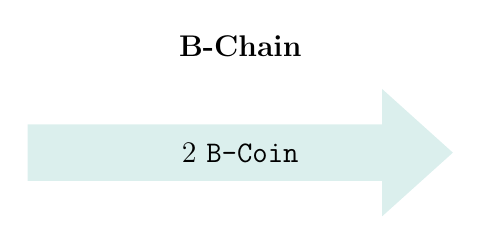
\begin{tikzpicture}[scale=0.9, every node/.style={scale=0.9}]
				\draw[color=black] plot (0,1.5) node {\large{{\textbf{B-Chain}}}};
				\fill[highlight!40] (-3,-0.4) -- (2,-0.4) -- (2,-.9) -- (3,0) -- (2,.9) -- 	(2,0.4) -- (-3, 0.4) -- (-3,-0.4);
				\draw[color=black] plot (0,0) node {\large{2 \texttt{B-Coin}}};
			\end{tikzpicture}
		\end{figure}
	\end{minipage}%
	\begin{minipage}{0.1\linewidth}
		\vspace{0.55cm}
		\centering
		\hspace{-0.2cm}
\includegraphics[width=1cm]{../assets/images/agents/handing_left}
		\\ \textbf{Bob}\\
		\vspace{0.3cm}
		\tikz{\filldraw[color = white!1] (0,0) rectangle ++(1cm,0.9cm);}
	\end{minipage}
\end{frame}

%%%

\begin{frame}{Atomic Cross Chain Swaps}
	\begin{minipage}{0.1\linewidth}
		\vspace{0.3cm}
		\centering
		
\includegraphics[width=1cm]{../assets/images/agents/handing_right}
		\\ \hspace{-0.3cm} \textbf{Alice}\\
		\vspace{0.3cm}
		\uncover<1->{
			\hspace{-0.2cm}	
\includegraphics[width=1cm]{../assets/images/hashlock_symbol}
		}
	\end{minipage}%
	\begin{minipage}{0.8\linewidth}
		\centering
	\vspace{0.3cm}
	\uncover<2->{
	\begin{figure}[t]
			\resizebox{0.6\linewidth}{!}{
			\begin{tikzpicture}[scale=0.9, every node/.style={scale=0.9}]
				\filldraw[yshift=-0.05cm, xshift=0.1cm,color = highlight!15, thick, 	draw=black, dashed] (-3,-5.8) rectangle ++(8cm,4.9cm);
				
				\draw[color=black] plot (1,-0.2) node [below]
				{\large{{\textbf{A-Chain}}}};
				
				% Inputs
				\draw[color=black] plot (-1,-1.65) node[above] {\texttt{inputs:}};
				
				% top left
				\filldraw[yshift=-0.05cm, xshift=0.1cm,color = highlight!25, thick, 	draw=highlight] (-2.6,-3.4) rectangle ++(3.3cm,1.8cm);
				\filldraw[yshift=-0.05cm, xshift=0.1cm,color = highlight!25, thick, 	draw=highlight] (-2.6,-3.4) rectangle ++(0.825cm,0.7cm);
				\draw[color=black] plot (-2.5,-2.25) node[right] {Bob:};
				\draw[color=black] plot (-1,-2.21)   node[right] {1 \texttt{A-Coin}};
				\draw[color=black] plot (-2.0875,-3.1)   node {\small{$Sig_B$}};
				
				\uncover<6->{\draw plot (-2.0875,-3.1) node {\checkmarkgreen};}
				
				% Outputs
				\draw[color=black] plot (3,-1.65)   node[above] {\texttt{outputs:}};
				
				% top right
				\filldraw[yshift=-0.05cm, xshift=0.1cm,color = highlight!25, thick, draw=highlight] (1.3,-5.4) rectangle ++(3.3cm,3.8cm);
				\draw[color=black, thick, dashed] (1.6,-3.75) -- (4.4,-3.75);	
				% top
				\filldraw[yshift=-0.05cm, xshift=0.1cm,color = highlight!25, thick, 	draw=highlight] (1.3,-3.4) rectangle ++(0.825cm,0.7cm);
				\filldraw[yshift=-0.05cm, xshift=0.1cm,color = highlight!25, thick, 	draw=highlight] (2.125,-3.4) rectangle ++(0.825cm,0.7cm);
				
				\draw[color=black] plot (1.4,-2.25)   node[right] {Alice:};
				\draw[color=black] plot (2.9,-2.21)   node[right] {1 \texttt{A-Coin}};
				\draw[color=black] plot (1.8125,-3.1)   node {\small{$Sig_A$}};
				\draw[color=black] plot (2.6375,-3.1)   node {
\includegraphics[width=0.5cm]{../assets/images/hashlock_symbol.png}};
				
				\uncover<7->{\draw plot (1.8125,-3.1) node {\checkmarkgreen};}
				\uncover<7->{\draw plot (2.6375,-3.1) node {\checkmarkgreen};}
				
				% bottom
				\uncover<3->{
				\filldraw[yshift=-0.05cm, xshift=0.1cm,color = highlight!25, thick,draw=highlight] (1.3,-5.4) rectangle ++(0.825cm,0.7cm);
				\filldraw[yshift=-0.05cm, xshift=0.1cm,color = highlight!25, thick,draw=highlight] (2.125,-5.4) rectangle ++(0.825cm,0.7cm);
				
				\draw[color=black] plot (1.4,-4.25)   node[right] {Bob:};
				\draw[color=black] plot (2.9,-4.21)   node[right] {1 \texttt{A-Coin}};
				\draw[color=black] plot (1.8125,-5.1)   node {\small{$Sig_B$}};
				\draw[color=black] plot (2.6375,-5.1)   node {
\includegraphics[width=0.5cm]{../assets/images/timelock_symbol.png}};}
			\end{tikzpicture}}
		\end{figure}
		\vspace{-0.4cm}
		\hspace{0.1cm}\tikz{\draw[color=black, thick, dashed] (-3,0) -- (3.5,0);}}
		\uncover<4->{
		\vspace{-0.2cm}
		\begin{figure}[b]
			\resizebox{0.6\linewidth}{!}{
			\begin{tikzpicture}[scale=0.9, every node/.style={scale=0.9}]
				\filldraw[yshift=-0.05cm, xshift=0.1cm,color = highlight!15, thick, 	draw=black, dashed] (-3,-5.8) rectangle ++(8cm,4.9cm);
				
				\draw[color=black] plot (1,-0.2) node [below]
				{\large{{\textbf{B-Chain}}}};
				
				% Inputs
				\draw[color=black] plot (-1,-1.65) node[above] {\texttt{inputs:}};
				
				% top left
				\filldraw[yshift=-0.05cm, xshift=0.1cm,color = highlight!25, thick, 	draw=highlight] (-2.6,-3.4) rectangle ++(3.3cm,1.8cm);
				\filldraw[yshift=-0.05cm, xshift=0.1cm,color = highlight!25, thick, 	draw=highlight] (-2.6,-3.4) rectangle ++(0.825cm,0.7cm);
				\draw[color=black] plot (-2.5,-2.25) node[right] {Alice:};
				\draw[color=black] plot (-1,-2.21)   node[right] {2 \texttt{B-Coin}};
				\draw[color=black] plot (-2.0875,-3.1)   node {\small{$Sig_A$}};
				
				\uncover<5->{\draw plot (-2.0875,-3.1) node {\checkmarkgreen};}
				
				% Outputs
				\draw[color=black] plot (3,-1.65)   node[above] {\texttt{outputs:}};
				
				% top right
				\filldraw[yshift=-0.05cm, xshift=0.1cm,color = highlight!25, thick, draw=highlight] (1.3,-5.4) rectangle ++(3.3cm,3.8cm);
				\draw[color=black, thick, dashed] (1.6,-3.75) -- (4.4,-3.75);	
				% top
				\filldraw[yshift=-0.05cm, xshift=0.1cm,color = highlight!25, thick, 	draw=highlight] (1.3,-3.4) rectangle ++(0.825cm,0.7cm);
				\filldraw[yshift=-0.05cm, xshift=0.1cm,color = highlight!25, thick, 	draw=highlight] (2.125,-3.4) rectangle ++(0.825cm,0.7cm);
				
				\draw[color=black] plot (1.4,-2.25)   node[right] {Bob:};
				\draw[color=black] plot (2.9,-2.21)   node[right] {2 \texttt{B-Coin}};
				\draw[color=black] plot (1.8125,-3.1)   node {\small{$Sig_B$}};
				\draw[color=black] plot (2.6375,-3.1)   node {
\includegraphics[width=0.5cm]{../assets/images/hashlock_symbol.png}};
						
				% bottom
				\filldraw[yshift=-0.05cm, xshift=0.1cm,color = highlight!25, thick,draw=highlight] (1.3,-5.4) rectangle ++(0.825cm,0.7cm);
				\filldraw[yshift=-0.05cm, xshift=0.1cm,color = highlight!25, thick,draw=highlight] (2.125,-5.4) rectangle ++(0.825cm,0.7cm);
				
				\draw[color=black] plot (1.4,-4.25)   node[right] {Alice:};
				\draw[color=black] plot (2.9,-4.21)   node[right] {2 \texttt{B-Coin}};
				\draw[color=black] plot (1.8125,-5.1)   node {\small{$Sig_A$}};
				\draw[color=black] plot (2.6375,-5.1)   node {
\includegraphics[width=0.5cm]{../assets/images/timelock_symbol_48.png}};
		\end{tikzpicture}}
	\end{figure}}
	\end{minipage}%
		\begin{minipage}{0.1\linewidth}
		\vspace{0.82cm}
		\centering
		\hspace{-0.2cm}
\includegraphics[width=1cm]{../assets/images/agents/handing_left}
		\\ \textbf{Bob}\\
		\vspace{0.3cm}
		\uncover<7->{
			
\includegraphics[width=1cm]{../assets/images/hashlock_symbol}
		}
	\end{minipage}
\end{frame}

%%%

\begin{frame}{Payment Channels}
	\begin{itemize}
		\item<1 -> Combination of timelocks, hashlocks and competitive outputs is very powerful.
		\item<2 -> Hash Time Locked Contracts are the basis of so-called payment channels.
		\item<3 -> The Bitcoin Blockchain (Layer 1) has scaling limitations. Payment channels tackle this, by allowing users to exchange transactions bilaterally, i.e. no need to add every single transaction to the Blockchain.
		\item<4 -> These transactions still benefit from the Blockchain's security and do not require trust. 
		\item<5 -> The next video will cover this topic in greater detail.
	\end{itemize}
\end{frame}

%%%

%\begin{frame}%[allowframebreaks]
%	\frametitle{References}
%	\bibliographystyle{amsplain}
%	\bibliography{../assets/bib/refs}
%\end{frame}

%%%

\end{document}